\documentclass[svgnames]{article}
\usepackage[utf8]{inputenc}
\usepackage{amsmath}
\usepackage{amssymb}
\usepackage{mathrsfs}
\usepackage{mathtools}
\newtheorem{mydef}{Given}
\newtheorem{mytheorem}{Theorem}
\usepackage{enumitem}
\usepackage{venndiagram}
\usepackage{smartdiagram}
\usepackage{caption}
\usepackage{subcaption}
%\usepackage[framed,numbered,autolinebreaks,useliterate]{mcode}
\usepackage{graphicx}
\graphicspath{ {./images/} }

\usepackage{listings}
\usepackage{color}

\definecolor{dkgreen}{rgb}{0,0.6,0}
\definecolor{gray}{rgb}{0.5,0.5,0.5}
\definecolor{mauve}{rgb}{0.58,0,0.82}

\lstset{frame=tb,
  language=Java,
  aboveskip=3mm,
  belowskip=3mm,
  showstringspaces=false,
  columns=flexible,
  basicstyle={\small\ttfamily},
  numbers=none,
  numberstyle=\tiny\color{gray},
  keywordstyle=\color{blue},
  commentstyle=\color{dkgreen},
  stringstyle=\color{mauve},
  breaklines=true,
  breakatwhitespace=true,
  tabsize=3
}

\renewcommand{\theenumi}{\Alph{enumi}}
\newenvironment{amatrix}[1]{%
  \left(\begin{array}{@{}*{#1}{c}|c@{}}
}{%
  \end{array}\right)
}

\newenvironment{tolerant}[1]{%
  \par\tolerance=#1\relax
}{%
  \par
}


\title{Statistical Methods: Homework 4}
\author{Cameron McIntyre}
\date{24 September, 2018}

\begin{document}

\maketitle

\section{3.10.4}
The complement of the event is P($Y_1$>.6)$\cup$P($Y_5$<.6).

These are disjoint events.

Therefore  P($Y_1$>.6)$\cup$P($Y_5$<.6)= P($Y_1$>.6) + P($Y_5$<.6).

And  P($Y_1$>.6) = $[P(Y<.6)]^5)$

$$ P(Y>.6)= \int_{.6}^{1}2y dy=(.64)^5  $$ $$   P(Y>.6) = .107$$

Also

$$ P(Y_5<.6) = (\int_{0}^{.6}2y dy)^5 = (.36)^5 $$ $$  P(Y_5<.6)  = .006$$

Therefore,

$$  P(Y_1<.6)\cup(Y_5>.6) = 1 - .107 - .006 = .887 $$

\section{3.10.6}

$f_Y(y)=e^{\lambda}$ And, $F_Y(y)=1-e^{\lambda}$


$$f(y_{min}<Y)=\int_{0}^{t} n \cdot f_Y(y)(1-F_Y(y))^{n-1}dy = \int_{0}^{t}ne^{-ny}dy$$

$$ f(y_{min}<Y)=-e^{-ny}\Big|^{t}_{0}=1-e^{-nt}$$

So using t=.2 and Probability = .9, we need to solve .9 $\leq 1- e^{-.2n}$.


This happens with n>11.5, so n should be greater than 12. $n\geq 12$

\section{3.10.8}

Find the pdf for $y_i$

$$f_{y_{i}}(y)=\frac{n!}{(i-1)!(n-i)!}F_y(y)^{i-1}(1-F_y(y))^{n-i}f_Y(y)dy $$

So, $f_Y(y) = 2y$ and $F_{Y}(y)=\frac{2y^2}{2}=y^2$

$$f_{y_{i}}(y)=\frac{n!}{(i-1)!(n-i)!}(y^2)^{i-1}(1-y^2)^{n-i} 2y dy$$

letting i = 5

$$f_{y_{5}}(y)=\frac{5!}{(5-1)!(5-5)!}(y^2)^{4}(1-y^2)^{5} 2y dy$$

$$f_{y_{5}}(y)=10y^{9}$$


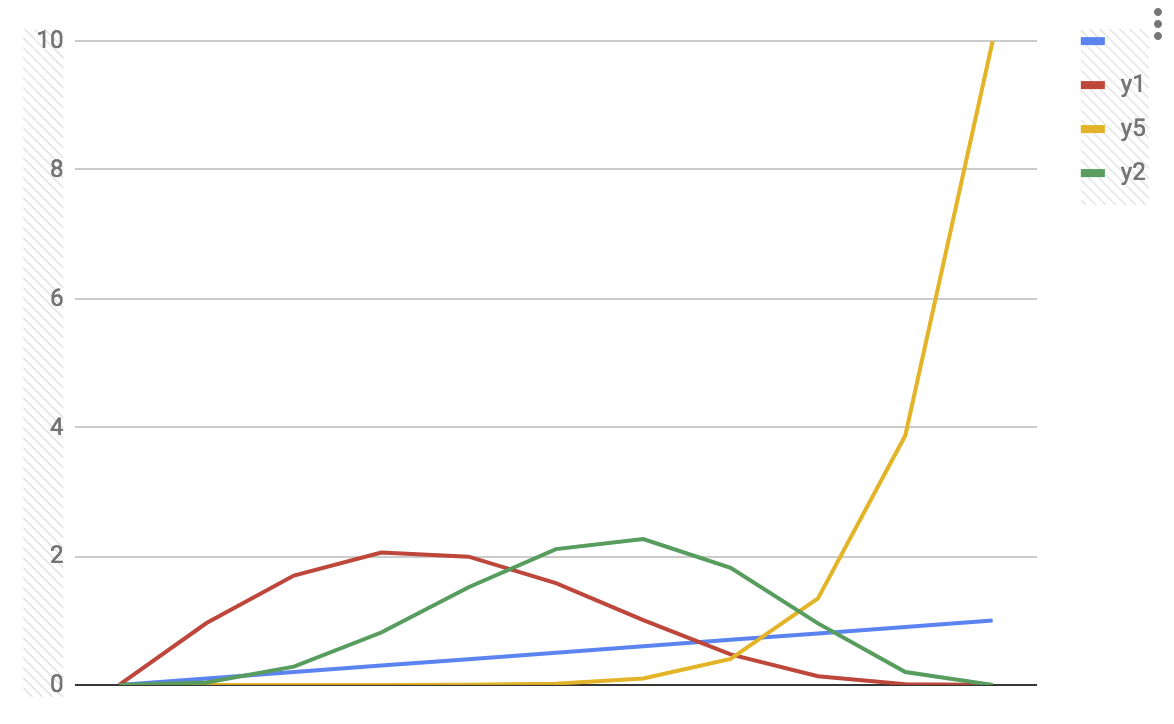
\includegraphics[scale=.65]{graphs}

\section{3.10.10}

So for the $N^{th}$ observation to be the smallest it must be smaller than each of the other observations in the sample. Being as they are identically distributed, the probability of any $Y_{i}$ being smaller or larger than another $Y_{j}$ is .5. That is $P(Y_{i}) > P(Y_{j})=.5$ and  $P(Y_{i}) < P(Y_{j})=.5$ for all $i \neq j$.

So there are n-i of these comparisons that have to happen, and there is only 1 way to arrange the samples. Therefore

$$P(Smallest \ Value \ in \ n^{th} spot) = (\frac{1}{2})^{n-1}$$


\section{3.10.12}

This question is essentially asking what is the expected value of the first order statistic. We have a formula for this: 

$$f_{y_{1}}(Y) = \int_{0}^{\infty}n F_{y}(Y)^0[1- F_{y}(Y)]^{n-1} f_{y}(y) dy$$

Simplify this and take the expected value.

$$ E[Y_1]  = \int_{0}^{\infty} n [1-e^{\lambda y}]^0 [e^{-\lambda y}]^{n-1} \lambda e^{-\lambda y} \cdot y dy$$

$$ E[Y_1]  = \int_{0}^{\infty} n \frac{[e^{-\lambda y}]^{n}}{e^{-\lambda y}} \lambda e^{-\lambda y} \cdot y dy$$

$$ E[Y_1]  = \int_{0}^{\infty} n \lambda e^{-(\lambda \cdot n) y}\cdot y dy$$

This is just an exponential distribution with parameter $\lambda^{'} = n \cdot \lambda$. Therefore we know the expected value of this distribution is $E[Y_1]  = \frac{1}{n \cdot \lambda}$, as required by the question, and as we have shown in a previous assignment.  

\section{3.12.4}

We have $p_x(k)=\frac{3}{4}^{k}\frac{1}{4}$. 

Therefore

$$ M_{x}(t)=\sum_{\infty}^{0}e^{tk}\frac{3}{4}^{k}\frac{1}{4}=\frac{1}{4}\sum_{0}^{\infty}(\frac{3e^t}{4})^k$$

$$\frac{1}{4}\sum_{0}^{\infty}(\frac{3e^t}{4})^k=\frac{1}{4} \cdot \frac{1}{1-\frac{3e^t}{4}}$$

So, $ M_{x}(t) = \frac{1}{4} \cdot \frac{1}{1-\frac{3e^t}{4}}$ and this converges when $e^t < \frac{4}{3}$.

\section{3.12.7}

To find the MGF we find $E[e^{tk}]$:

$$ E[e^{tk}] = \sum_{0}^{\infty} e^{-\lambda} e^{tk}\frac{\lambda^{k}}{k!}=\frac{1}{e^{\lambda}}\sum_{0}^{\infty} \frac{(\lambda t)^k}{k!} = \frac{e^{t \lambda}}{e^\lambda}=e^{\lambda(t-1)}$$

\section{3.12.10}

Find $E[Y^4]$ of $y~ exp(\lambda), y > 0$.

We find the MGF of the exponential distribution

$$ \int_{0}^{\infty} e^{ty}\lambda e^{-\lambda y} dy =  \int_{0}^{\infty} \lambda e^{-(\lambda-t) y}dy$$

We substitute $(\lambda - t)y=u$ in the integral. So $\frac{du}{\lambda - t}= dy$. And so,

$$MGF = \frac{\lambda}{\lambda-t}(-e^{-u})\big|^{u=\infty}_{u=0}=  \frac{\lambda}{\lambda-t}(0-(-1))= \frac{\lambda}{\lambda-t}$$

No we go through the thrilling exercise of taking repeated partial derivatives 4 times of this MGF.

$$\frac{d}{dt}\frac{\lambda}{\lambda-t}=\lambda(\lambda-t)^{-2} $$

$$\frac{d^2f}{dt^2}=\frac{d}{dt}\frac{df}{dt}=2\lambda(\lambda-t)^-3 $$

From this we can see the pattern that the nth moment is $n!\frac{\lambda}{{(\lambda-t)^{n+1}}}$

Therefore the forth moment is: $24\frac{\lambda}{(\lambda-t)^{5}}$

Evaluating this at t=0, $E[Y^4]=\frac{24}{\lambda^5}$

\section{3.12.23}

$X - poi(\lambda)$, and $f_x(x) = e^{-\lambda}\frac{\lambda^x}{x!}$

Also,

$M_x(t)=e^{-\lambda + \lambda e^{t}}$
\newline
\newline
\newline
a) We consider $W=3X$.

Then,

$$ M_{W}(t) = M_{X}(3t) = e^{(\lambda  (e^{(3t) - 1)})}.$$

Based on this result we see W is not distributed as a poisson with a parameter because the MGF doesn't match what we would expect to see.
So, in response to part a, No $W - Poi(\lambda^{'})$
\newline
\newline
\newline
b) We consider $W_2=3X+1$.

We know $M_W(t)=e^{-3\lambda + 3\lambda e^{t}}$ from part a.

So $M_{W_{2}}=e^t \cdot e^{-3\lambda + 3\lambda e^{t}}$.

This is not a Poisson moment generating function. Therefore it is not distributed as a poisson random Variable. 


\section{R Programming assignment}

\textbf{Part 1:}
\begin{lstlisting}


event_1 <- 0
invcdf <- function(y) sqrt(y)
for (i in 1:1000){
  res<-sort(invcdf(runif(5)))
  if (res[1] < .6){
    if (res[5]>.6){
      event_1=event_1+1
    }
    else{
      warning("5th not greater than .6")
    }
  }
  else{
    warning("1st not less than .6")
  }
}
 
 
 j = event_1/1000
\end{lstlisting}
The value of J is .885. This is very close to our theoretical value of .887.

\textbf{Part 2:}

\begin{lstlisting}
event_2 <- 0
invcdf_two <- function(y) -log((1 - y))

for (i in 1:1000){
  res_one <- sort(invcdf_two(runif(12)))[1]
  if (res_one < .2){
    event_2 = event_2 + 1
  }
}

\end{lstlisting}

The value of event\_2 is 911. So, .911 is the calculated probability, which is close to our expected value of .9 which we found analytically.

\end{document}